\documentclass[twocolumn,9pt]{sigplanconf}

\usepackage{url}
% \usepackage{code}
\usepackage{graphicx}
\usepackage{enumerate}

\usepackage{listings}
\lstset{basicstyle=\fontfamily{cmss} \small, columns=fullflexible, language=Haskell, numbers=left, numberstyle=\tiny, numbersep=2pt}

\newcommand{\codef}[1]{{\fontfamily{cmss}\small#1}}
\newcommand{\boldcode}[1]{{\bf\fontfamily{cmss}\small#1}}

\usepackage{natbib}
\bibpunct();A{},
\let\cite=\citep

\nocaptionrule

\title{Parallel Performance Tuning for Haskell}

\authorinfo{Donnie Jones}{University of Kentucky}
           {donnie@darthik.com}
\authorinfo{Simon Marlow}{Microsoft Research}
           {simonmar@microsoft.com}
\authorinfo{Satnam Singh}{Microsoft Research}
           {satnams@microsoft.com}

\begin{document}

\maketitle
%\makeatactive

\begin{abstract}
Parallel Haskell programming has entered the mainstream with support
now included in GHC for multiple parallel programming models, along
with multicore execution support in the runtime.  However, tuning
programs for parallelism is still something of a black art.  Without
much in the way of feedback provided by the runtime system, it is a
matter of trial and error combined with experience to achieve good
parallel speedups.

This paper describes an early prototype of a parallel profiling system
for multicore programming with GHC.  The system comprises three parts:
fast event tracing in the runtime, a Haskell library for reading the
resulting trace files, and a number of tools built on this library for
presenting the information to the programmer.  We focus on one tool in
particular, a graphical timeline browser called ThreadScope.

The paper illustrates the use of ThreadScope through a number of case
studies, and describes some useful methodologies for parallelising
Haskell programs.
\end{abstract}


\section{Introduction}

Life has never been better for the Parallel Haskell programmer: GHC
supports multicore execution out of the box, including multiple
parallel programming models: Strategies \cite{spj:trin98b}, Concurrent
Haskell \cite{jones96concurrent} with STM \cite{stm}, and Data Parallel Haskell
\cite{dph}.  Performance of the runtime system has received 
attention recently, with significant improvements in parallel
performance available in the forthcoming GHC release \cite{multicore-ghc}.
Many of the runtime bottlenecks that hampered parallel performance in
earlier GHC versions are much reduced, with the result that it should
now be easier to achieve parallel speedups.

However, optimising the runtime only addresses half of the problem;
the other half being how to tune a given Haskell program to run
effectively in parallel.  The programmer still has control over task
granularity, data dependencies, speculation, and to some extent
evaluation order.  Getting these wrong can be disastrous for parallel
performance. For example the granularity should neither be too fine
nor too coarse.  The runtime does everything it can to broaden the
range of granularities that yield good performance, but it cannot
completely eliminate the upper and lower bounds.

Current methods for tuning parallel Haskell programs rely largely on
trial and error, experience, and an eye for understanding the limited
statistics produced at the end of a program's run by the runtime
system.  What we need are effective ways to measure and collect
information about the runtime behaviour of parallel Haskell programs,
and tools to communicate this information to the programmer in a
way that they can understand and use to solve performance problems
with their programs.

In this paper we describe a new profiling system developed for the
purposes of understanding the parallel execution of Haskell programs.
In particular, our system includes a tool called ThreadScope that
allows the programmer to interactively browse the parallel execution
profile.

This paper contributes the following:

\begin{itemize}
\item We describe the design of our parallel profiling system, and
  the ThreadScope tool for understanding parallel execution.  Our
  trace file format is fully extensible, and profiling tools built
  using our framework are both backwards- and forward-compatible with
  different versions of GHC.

\item Through several case studies, we explore how to use ThreadScope
  for identifying parallel performance problems, and describe a
  selection of methodologies for parallelising Haskell code.
\end{itemize}

Earlier methodologies for parallelising Haskell code exist
\cite{spj:trin98b}, but there are two crucial differences in the
multicore GHC setting.  Firstly, the trade-offs are likely to be
different, since we are working with a shared-memory heap, and
communication is therefore cheap\footnote{though not entirely free,
  since memory cache hierarchies mean data still has to be shuffled
  between processors even if that shuffling is not explicitly
  programmed.}.  Secondly, it has recently been discovered that
Strategies interact badly with garbage collection
\cite{multicore-ghc}, so in this paper we avoid the use of the
original Strategies library, relying instead on our own simple
hand-rolled parallel combinators.

Our work is at an early stage.  The ThreadScope tool displays only one
particular view of the execution of Parallel Haskell programs (albeit
a very useful one).  There are a wealth of possibilities, both for
improving ThreadScope itself and for building new tools.  We cover
some of the possibilities in Section~\ref{s:conclusion}.

\section{Profiling Motivation}
Show examples of semi-explicit parallel programs that go wrong. Show what we could measure before using heap and time profiling and motivate the need for better profiling.

Haskell provides a mechanism to allow the user to control the granularity of parallelism by indicating what computations may be usefully carried out in parallel. This is done by using functions from the \codef{Control.Parallel} module. The interface for \codef{Control.Parallel} is shown below:
\begin{lstlisting}
  par :: a -> b -> b 
  pseq :: a -> b -> b 
\end{lstlisting}
The function \codef{par} indicates to the GHC run-time system that it may be beneficial to evaluate the first argument in parallel with the second argument. The \codef{par} function returns as its result the value of the second argument. One can always eliminate \codef{par} from a program by using the following identity without altering the semantics of the program:
\begin{lstlisting}
  par a b = b 
\end{lstlisting}
A thread is not necessarily created to compute the value of the expression \codef{a}. Instead, the GHC run-time system creates a {\em spark} which has the potential to be executed on a different thread from the parent thread. A sparked computation expresses the possibility of performing some speculative evaluation. Since a thread is not necessarily created to compute the value of \codef{a} this approach has some similarities with the notion of a {\em lazy future}~\cite{mohr:91}.

Sometimes it is convenient to write a function with two arguments as an infix function and this is done in Haskell by writing quotes around the function:
\begin{lstlisting}
  a `par` b
\end{lstlisting}

We call such programs semi-explicitly parallel because the programmer has provided a hint about the appropriate level of granularity for parallel operations and the system implicitly creates threads to implement the concurrency. The user does not need to explicitly create any threads or write any code for inter-thread communication or synchronization.

To illustrate the use of \codef{par} we present a program that performs two compute intensive functions in parallel. The first compute intensive function we use is the notorious Fibonacci function:
\begin{lstlisting}
fib :: Int -> Int
fib 0 = 0
fib 1 = 1
fib n = fib (n-1) + fib (n-2)
\end{lstlisting}
The second compute intensive function we use is the \codef{sumEuler} function taken from~\cite{trinder:02}:
\begin{lstlisting}
mkList :: Int -> [Int]
mkList n = [1..n-1]

relprime :: Int -> Int -> Bool
relprime x y = gcd x y == 1

euler :: Int -> Int
euler n = length (filter (relprime n) (mkList n))

sumEuler :: Int -> Int
sumEuler = sum . (map euler) . mkList
\end{lstlisting}
The function that we wish to parallelize adds the results of calling \codef{fib} and \codef{sumEuler}:
\begin{lstlisting}
sumFibEuler :: Int -> Int -> Int
sumFibEuler a b = fib a + sumEuler b
\end{lstlisting}
As a first attempt we can try to use \codef{par} the speculatively spark off the computation of \codef{fib} while the parent thread works on \codef{sumEuler}:
\begin{lstlisting}
-- A wrong way to parallelize f + e
parSumFibEuler :: Int -> Int -> Int
parSumFibEuler a b
  = f `par` (f + e)
    where
    f = fib a
    e = sumEuler b
\end{lstlisting}

To create two workloads that take roughly the same amount of time to execute we performed some experiments which show that \codef{fib 38} takes roughly the same time to execute as \codef{sumEuler 5300}. If we were to run this program and view the execution trace we would see somthing like the graph shown in Figure~\ref{f:wrongpar}.

\begin{figure}
\begin{center}
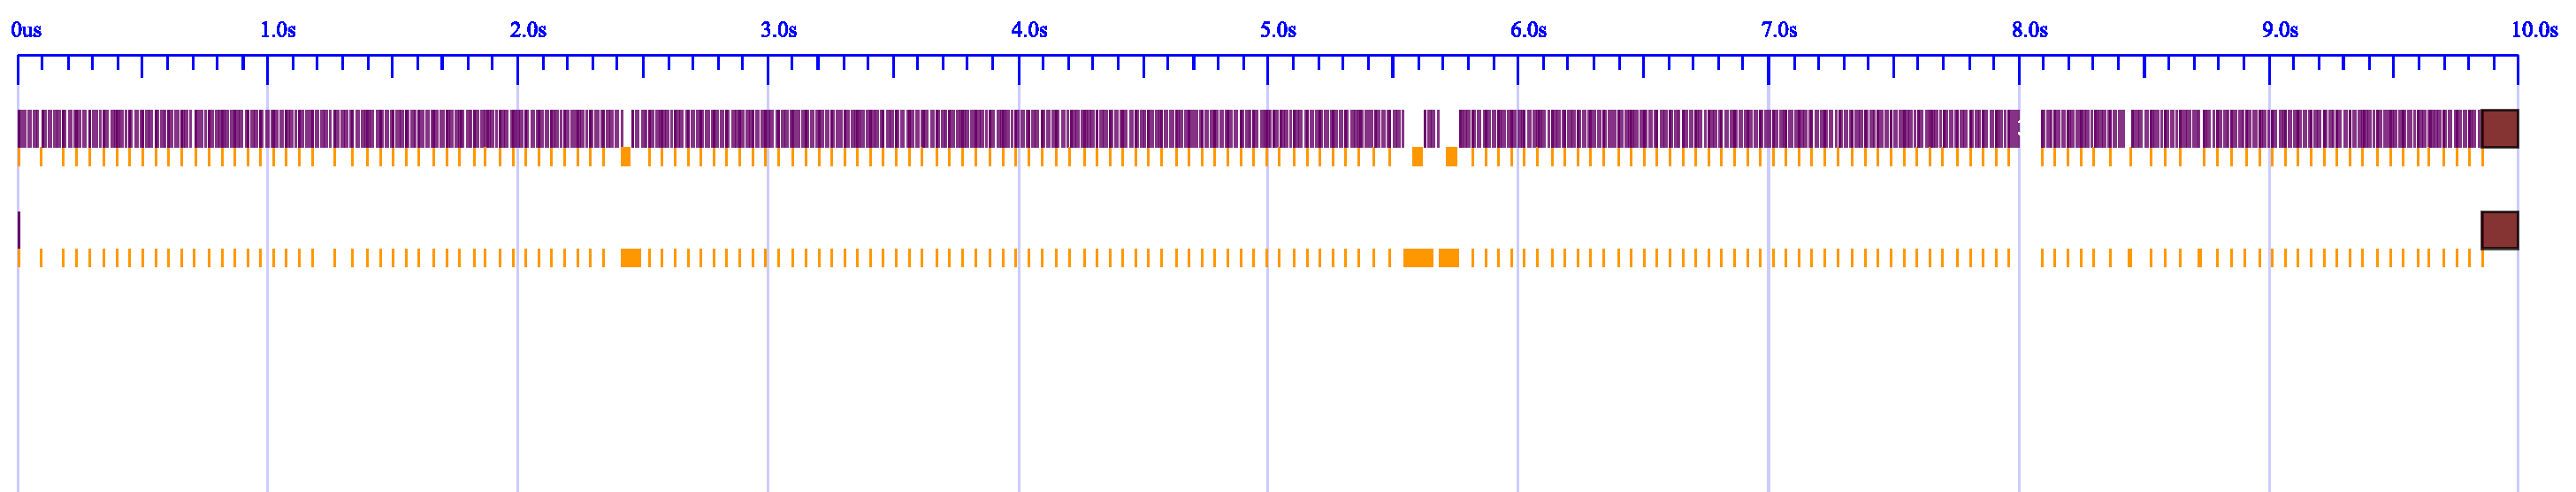
\includegraphics[width=8.5cm]{SumEuler1-N2-eventlog.pdf}
\end{center}
\caption{No parallelization of \codef{f `par` (f + e)}}
\label{f:wrongpar}
\end{figure}

We can examine an execution log to help understand what went wrong:

\begin{verbatim}
  SPARKS: 1 (0 converted, 0 pruned)

  INIT  time    0.00s  (  0.00s elapsed)
  MUT   time    9.39s  (  9.61s elapsed)
  GC    time    0.37s  (  0.24s elapsed)
  EXIT  time    0.00s  (  0.00s elapsed)
  Total time    9.77s  (  9.85s elapsed)
\end{verbatim}

The log shows that although a spark was created for the potential parallel evaluation of \codef{fib 38} it was never picked up for evaluation. In this case the performance bug is due to the fact that the main thread immediately starts to work on the evaluation of \codef{fib 38} itself which causes this spark to fizzle. One might be tempted to fix this problem by swapping the arguments to the \codef{+} operator in the hope that the main thread will work on \codef{sumEuler} while the sparked thread works on \codef{fib}:

\begin{lstlisting}
-- Maybe a lucky parallelization
parSumFibEuler :: Int -> Int -> Int
parSumFibEuler a b
  = f `par` (e + f)
    where
    f = fib a
    e = sumEuler b
\end{lstlisting}

This results in the execution trace shown in Figure~\ref{f:lucky} which shows a sparked thread being taken up by a spare worker thread. 

\begin{figure}
\begin{center}
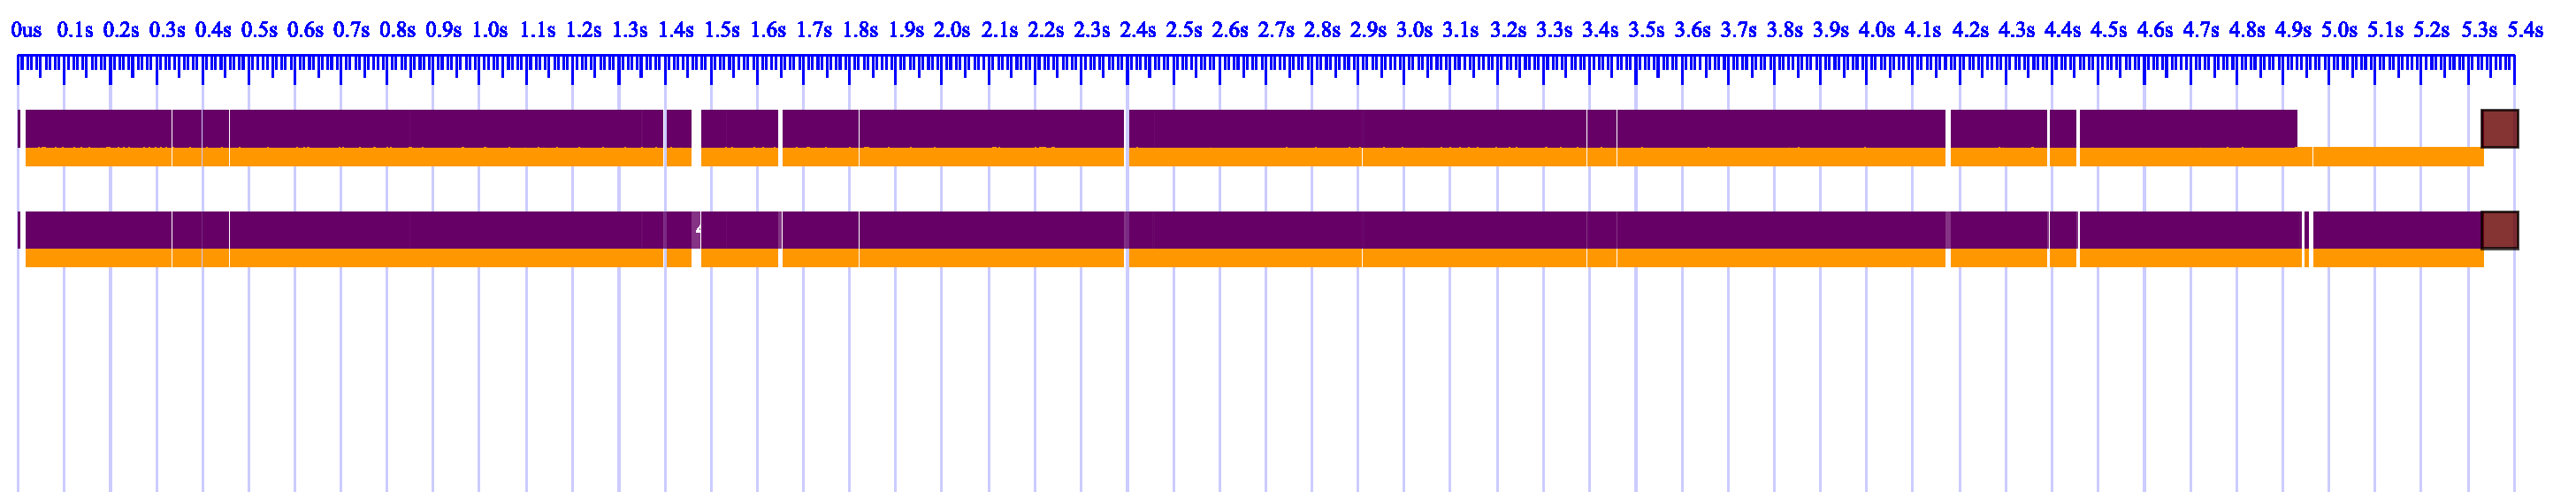
\includegraphics[width=8.5cm]{SumEuler2-N2-eventlog.pdf}
\end{center}
\caption{A luck parallelization of \codef{f `par` (e + f)}}
\label{f:wrongpar}
\end{figure}

The execution log for this program shows that a spark was used productively and the elapsed time has dropped from 9.85s to 5.33s:

\begin{verbatim}
  SPARKS: 1 (1 converted, 0 pruned)

  INIT  time    0.00s  (  0.00s elapsed)
  MUT   time    9.47s  (  4.91s elapsed)
  GC    time    0.69s  (  0.42s elapsed)
  EXIT  time    0.00s  (  0.00s elapsed)
  Total time   10.16s  (  5.33s elapsed)
\end{verbatim}

The better way to evaluate \codef{fib} and \codef{sumEuler} in parallel is to used the \codef{pseq} combinator to ensure that the main thread works on \codef{suMEuler} while the sparked thread works on \codef{fib}:

\begin{lstlisting}
-- A correct parallelization that does not depend on
-- the evaluation order of +
parSumFibEuler :: Int -> Int -> Int
parSumFibEuler a b
  = f `par` (e `pseq` (f + e))
    where
    f = fib a
    e = sumEuler b
\end{lstlisting}

This version does not make any assumptions about the evaluation order of \codef{+} which is undefined in Haskell.


\section{Profiling Infrastructure}
Our profiling framework comprises three parts:

\begin{itemize}
\item Support in GHC's runtime for tracing events to a log file at
  runtime.  The tracing is designed to be as lightweight as possible,
  so as not to have any significant impact on the behaviour of the
  program being measured.

\item A Haskell library \codef{ghc-events} that can read the trace file
  generated by the runtime and build a Haskell data structure
  representing the trace.

\item Multiple tools make use of the \codef{ghc-events} library to read and
  analyse trace files.
\end{itemize}

Having a single trace-file format and a library that parses it means
that it is easy to write a new tool that works with GHC trace files:
just import the \codef{ghc-events} package and write code that uses the
Haskell data structures directly.  We have already built several such
tools ourselves, some of which are merely proof-of-concept
experiments, but the \codef{ghc-events} library makes it almost trivial to
create new tools:

\begin{itemize}
\item A simple program that just prints out the (sorted) contents of
  the trace file as text.  Useful for checking that a trace file can
  be parsed, and for examining the exact sequence of events.

\item The ThreadScope graphical viewer.

\item A tool that parses a trace file and generates a PDF format
  timeline view, similar to the ThreadScope view.

\item A tool that generates input in the format expected by the
  gtkwave circuit waveform viewer.  This was used as an early
  prototype for ThreadScope, since the timeline view that we want to
  display has a lot in common with the waveform diagrams that gtkwave
  displays and browses.
\end{itemize}

\subsection{Fast runtime tracing}
Minimizing the overhead of event logging is critical when designing a system
to facilitate runtime tracing.  In the GHC runtime, a pre-allocated events buffer is 
used by each HEC to store generated events.
By doing so, we prevent any performance delays from dynamic 
memory allocation, and require no locks since the buffers are
HEC-local.  Yet, this requires us to flush the buffer
to the filesystem once it becomes full, but since the buffer is a
fixed size we pay a near-constant penalty for each flush and a
deterministic delay on the GHC runtime.

The HEC-local buffers are flushed independently, which means that
events in the log file appear out-of-order and have to be sorted.
Sorting of the events is easily performed by the profiling tool after
reading in the log file using the \codef{ghc-events} library.

To measure the speed at which the GHC runtime can log events, we used
a C program (no Haskell code, just using the GHC runtime system as a
library) that simply generates 2,000,000 events, alternating between
``thread start'' and ``thread stop'' events.  Our program generates a
34MB trace file and runs in 0.31 seconds elapsed time:

\begin{figure*}
\begin{center}
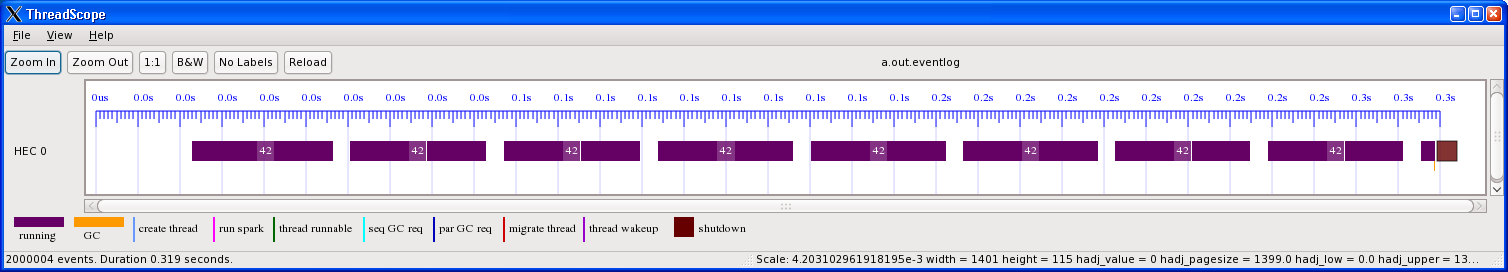
\includegraphics[scale=0.3]{eventbench.png}
\end{center}
\caption{Synthetic event benchmark}
\label{f:event-bench}
\end{figure*}

\begin{verbatim}
  INIT  time    0.00s  (  0.02s elapsed)
  MUT   time    0.22s  (  0.29s elapsed)
  GC    time    0.00s  (  0.00s elapsed)
  EXIT  time    0.00s  (  0.00s elapsed)
  Total time    0.22s  (  0.31s elapsed)
\end{verbatim}
which gives a rough figure of 150ns for each event on average.
Looking at the ThreadScope view of this program
(Figure~\ref{f:event-bench}) we can clearly see where the buffer
flushes are happening, and that each one is about 5ms long.

An alternative approach is to use memory-mapped files, and write our
events directly into memory, leaving the actual file writing to the
OS.  This would allow writing to be performed asynchronously, which
would hopefully reduce the impact of the buffer flush.  According to
\codef{strace} on Linux, the above test program is spending 0.7s
writing buffers, so making this asynchronous would save us about 30ns
per event on average.  However, on a 32-bit machine where we can't
afford to reserve a large amount of address space for the whole log
file, we would still have to occasionally flush and remap new portions
of the file.  This alternative approach is something we plan to
explore in the future.

% how much impact does this have on runtimes?
To see how much impact event logging has on real execution times, we
took a parallel version of the canonical Fibonacci function,
\codef{parfib}, and compared the time elapsed with and without event
logging enabled for 50 executions of parfib on an Intel(R) Core(TM)2
Duo CPU T5250 1.50GHz, using both cores.  The program generates about
2,000,000 events during the run, and generates a 40MB log file.

\begin{verbatim}
  parfib eventlog 
  ./Main 40 10 +RTS -N2 -l -RTS
  Avg Time Elapsed  Standard Deviation
  20.582757s        0.789547s

  parfib without eventlog 
  ./Main 40 10 +RTS -N2 -RTS
  Avg Time Elapsed  Standard Deviation
  17.447493s        1.352686s
\end{verbatim}

Considering the significant number of events generated in the traces
and the very detailed profiling information made available by these
traces, the overhead does not have an immense impact at approximately
10-25\% increase in elapsed time.  In the case of parfib, the event
representing the creation of a new spark is dominant, comprising at
least 80\% of the the events generated.  In fact, it is debatable
whether we should be logging the creation of a spark, since the cost
of logging this event is likely to be larger than the cost of creating
the spark itself - a spark creation is simply a write into a circular
buffer.
  
For parallel quicksort, far fewer sparks are created and most of the
computation is spent in garbage collection; thus, we can achieve an
almost unnoticeable overhead from event tracing.  The parallel quicksort
example involved sorting a list of 100,000 randomly generated integers
and was performed in the same manner as parfib where we compare with
event logging and without, yet in this test we perform 100 executions 
on an Intel(R) Core(TM) 2 Quad CPU 3.0Ghz. 

\begin{verbatim}
  parquicksort eventlog 
  ./Main +RTS -N4 -l -RTS 
  Avg Time Elapsed  Standard Deviation
  14.201385s        2.954869

  parquicksort without eventlog 
  ./Main +RTS -N4 -RTS 
  Avg Time Elapsed  Standard Deviation
  15.187529s        3.385293s

\end{verbatim}

Since parallel quicksort spent the majority of the computation doing
useful work, particularly garbage collection of the created lists, a
trace file of only approximately 5MB and near 300,000 events was
created and the overhead of event tracing is not noticeable.

The crux of the event tracing is that even when a poorly performing
program utilizes event tracing, the overhead should still not be
devastating to the program's performance, but best of all on a program
with high utilization event tracing should barely affect the performance.

\subsection{An extensible file format}

We believe it is essential that the trace file format is both
backwards and forwards compatible, and architecture independent.  In
particular, this means that:

\begin{itemize}
\item If you build a newer version of a tool, it will still work with
  the trace files you already have, and trace files generated by
  programs compiled with older versions of GHC.

\item If you upgrade your GHC and recompile your programs, the trace
  files will still work with any profiling tools you already have.

\item Trace files do not have a shelf life.  You can keep your trace
  files around, safe in the knowledge that they will work with future
  versions of profiling tools.  Trace files can be archived, and
  shared between machines.
\end{itemize}

Nevertheless, we don't expect the form of trace files to remain
completely static.  In the future we will certainly want to add new
events, and add more information to existing events.  We therefore
need an extensible file format.  Informally, our trace files are
structured as follows:

\begin{itemize}
\item A list of \emph{event types}.  An event-type is a
  variable-length structure that describes one kind of event.  The
  event-type structure contains
  \begin{itemize}
    \item A unique number for this event type
    \item A field describing the length in bytes of an instance of the
      event, or zero for a variable-length event.
    \item A variable-length string (preceded by its length) describing
      this event (for example ``thread created'')
    \item A variable-length field (preceded by its length) for future
      expansion.  We might in the future want to add more fields to
      the event-type structure, and this field allows for that.
  \end{itemize}
\item A list of \emph{events}.  Each event begins with an event number
  that corresponds to one of the event types defined earlier, and the
  length of the event structure is given by the event type (or it has
  variable length).  The event also contains
  \begin{itemize}
  \item A nanosecond-resolution timestamp.
  \item For a variable-length event, the length of the event.
  \item Information specific to this event, for example which CPU it
    occurred on.  If the parser knows about this event, then it can
    parse the rest of the event's information, otherwise it can skip
    over this field because its length is known.
  \end{itemize}
\end{itemize}

The unique numbers that identify events are shared knowledge between
GHC and the \codef{ghc-events} library.  When creating a new event, a new
unique identifier is chosen; identifiers can never be re-used.

Even when parsing a trace file that contains new events, the parser
can still give a timestamp and a description of the unknown events.
The parser might encounter an event-type that it knows about, but the
event-type might contain new unknown fields.  The parser can recognise
this situation and skip over the extra fields, because it knows the
length of the event from the event-type structure.  Therefore when a
tool encounters a new log file it can continue to provide consistent
functionality.

Of course, there are scenarios in which it isn't possible to provide
this ideal graceful degradation.  For example, we might construct a
tool that profiles a particular aspect of the behaviour of the
runtime, and in the future the runtime might be redesigned to behave
in a completely different way, with a new set of events.  The old
events simply won't be generated any more, and the old tool won't be
able to display anything useful with the new trace files.  Still, we
expect that our extensible trace file format will allows us to smooth
over the majority of forwards- and backwards-compatibility issues that
will arise between versions of the tools and GHC runtime.  Moreover,
extensibility costs almost nothing, since the extra fields are all in
the event-types header, which has a fixed size for a given version of
GHC.

\section{Case Studies}

\subsection{Batcher's Biotonic Parallel Sorter}
Batcher's bitonic merger and sorter is a parallel sorting algorithm which has a good implementation in hardware. We have produced an implementaiton of this algorithm in Haskell originally for circuit generation for FPGAs. However, this executable model also represents an interesting software implicit parallelization exercise because the entire parallel structure of the algorithm is expressed in terms of just one combinator called \codef{par2}:

\begin{lstlisting}
par2 :: (a -> b) -> (c -> d) -> (a, c) -> (b, d)
par2 circuit1 circuit2 (input1, input2)
  = (output1, output2)
    where
    output1 = circuit1 input1
    output2 = circuit2 input2
\end{lstlisting}

This combinator captures the idea of two circuits which are independent and execute in parallel. A straight-forward way to perform a semi-explicit parallelization of this function is use \codef{par} to spark off the evaluation of one of the sub-circuits.

\begin{lstlisting}
par2 :: (a -> b) -> (c -> d) -> (a, c) -> (b, d)
par2 circuit1 circuit2 (input1, input2)
  = output1 `par` (output2 `pseq` (output1, output2))
    where
    output1 = circuit1 input1
    output2 = circuit2 input2
\end{lstlisting}

This relatively simple change results in a definate performance gain due to parallelsim. Here is the log output produced by running a test-bench program with just one Haskell execution context:

\begin{verbatim}
.\bsortpar.exe +RTS -N1 -l -qg0 -qb -sbsortpar-N1.log
  SPARKS: 106496 (0 converted, 106496 pruned)

  INIT  time    0.00s  (  0.00s elapsed)
  MUT   time    5.32s  (  5.37s elapsed)
  GC    time    0.72s  (  0.74s elapsed)
  EXIT  time    0.00s  (  0.00s elapsed)
  Total time    6.04s  (  6.12s elapsed)
\end{verbatim}

Although many sparks are created non are taken up because there is only one worker thread. The execution trace for this invocation is shown in Figure~\ref{f:bsortpar-n1}.

\begin{figure*}
\begin{center}
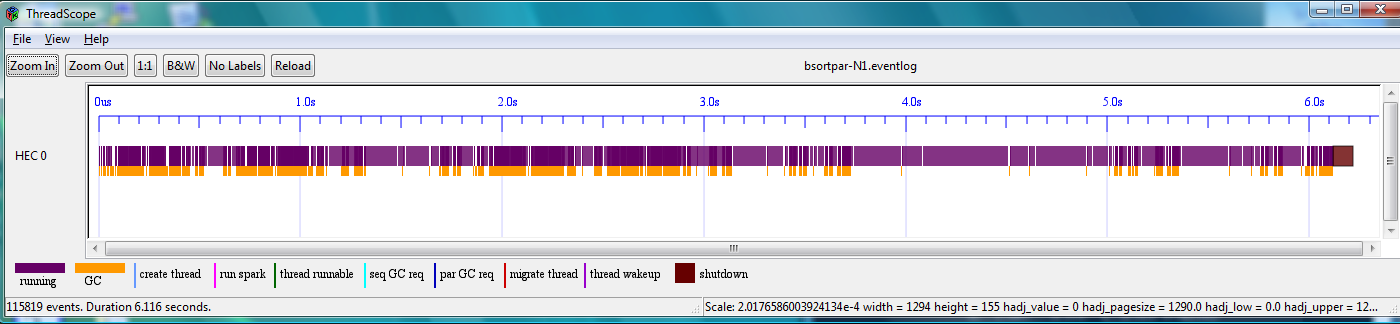
\includegraphics[width=17cm]{bsortpar-n1.png}
\end{center}
\caption{A sequential execution of bsort}
\label{f:bsortpar-n1}
\end{figure*}

Running with two threads shows a very good performance improvement:

\begin{verbatim}
$ cat bsortpar-N2.log
.\bsortpar.exe +RTS -N2 -l -qg0 -qb -sbsortpar-N2.log
  SPARKS: 106859 (49 converted, 106537 pruned)

  INIT  time    0.00s  (  0.00s elapsed)
  MUT   time    4.73s  (  3.03s elapsed)
  GC    time    1.64s  (  0.72s elapsed)
  EXIT  time    0.00s  (  0.00s elapsed)
  Total time    6.36s  (  3.75s elapsed)
\end{verbatim}

This example produces very many sparks most of which fizzle but enough sparks are turned into productive work i.e. 6.36 seconds worth of work done in 3.75 seconds of time. The execution trace for this invocation is shown in Figure~\ref{f:bsortpar-n2}. There is an obvious sequential block of execution between 2.1 seconds and 2.9 seconds and we believe this is due to a sequential component of the algorithm which combines the results of parallel sub-computations.

\begin{figure*}
\begin{center}
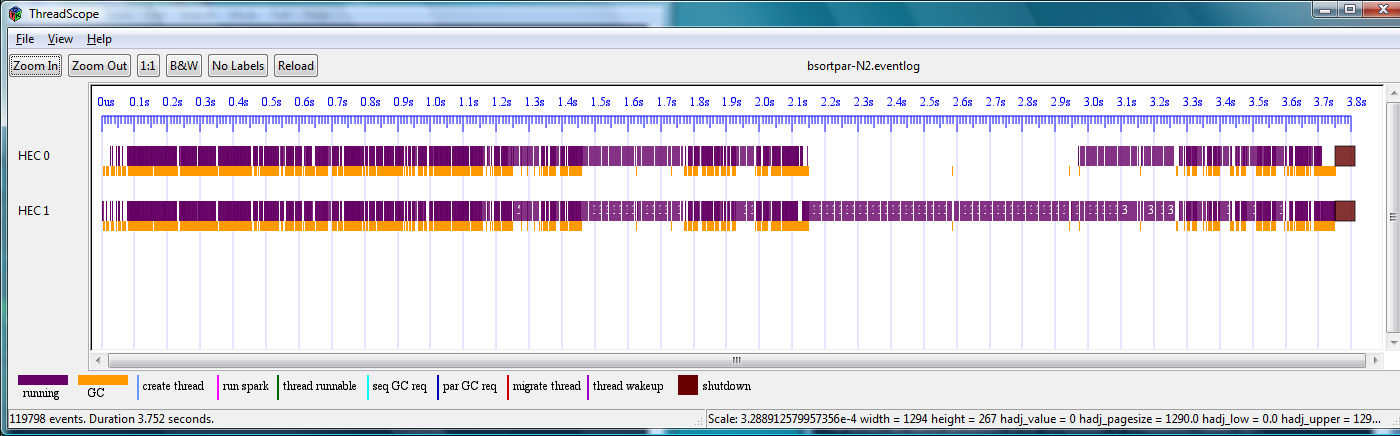
\includegraphics[width=17cm]{bsortpar-n2.png}
\end{center}
\caption{A parallel execution of bsort}
\label{f:bsortpar-n2}
\end{figure*}



\subsection{Soda}

Soda is a program for solving word-search problems: given a
rectangular grid of letters, find occurrences of a words from a
supplied list, where a word can appear horizontally, vertically, or
diagonally, in either direction (giving a total of eight possible
orientations).

The program has a long history as a Parallel Haskell benchmark
\cite{soda}.  The version we start with here is a recent incarnation,
using a random initial grid with a tunable size.  The words do not in
fact appear in the grid; the program just fruitlessly searches the
entire grid for a predefined list of words.  One advantage of this
formulation for benchmark purposes is that the program's performance
does not depend on the search order, however a disadvantage is that
the parallel structure is unrealistically regular.

The parallelism is expressed using \codef{parListWHNF} to avoid the
space leak issues with the standard strategy implementation of
\codef{parList} \cite{multicore-ghc}.  The \codef{parListWHNF}
function is straightforwardly defined thus:

\begin{verbatim}
parListWHNF :: [a] -> ()
parListWHNF [] = ()
parListWHNF (x:xs) = x `par` parListWHNF xs
\end{verbatim}

To establish the baseline performance, we run the program using GHC's
\texttt{+RTS -s} flags, below is an excerpt of the output:

\begin{verbatim}
  SPARKS: 12 (12 converted, 0 pruned)

  INIT  time    0.00s  (  0.00s elapsed)
  MUT   time    7.27s  (  7.28s elapsed)
  GC    time    0.61s  (  0.72s elapsed)
  EXIT  time    0.00s  (  0.00s elapsed)
  Total time    7.88s  (  8.00s elapsed)
\end{verbatim}

We can see that there are only 12 sparks generated by this program: in
fact the program creates one spark per word in the search list, of
which there are 12.  This rather coarse granularity will certainly
limit the ability of the runtime to effectively load-balance as we
increase the number of cores, but that won't be an issue with a small
number of cores.

Initially we try with 4 cores, and with GHC's parallel GC enabled:

\begin{verbatim}
  SPARKS: 12 (11 converted, 0 pruned)

  INIT  time    0.00s  (  0.00s elapsed)
  MUT   time    8.15s  (  2.21s elapsed)
  GC    time    4.50s  (  1.17s elapsed)
  EXIT  time    0.00s  (  0.00s elapsed)
  Total time   12.65s  (  3.38s elapsed)
\end{verbatim}

Not bad: 8.00/3.38 is a speedup of around 2.4 on 4 cores.  But since
this program has a highly parallel structure, we might hope to do
better.  

\begin{figure*}
\begin{center}
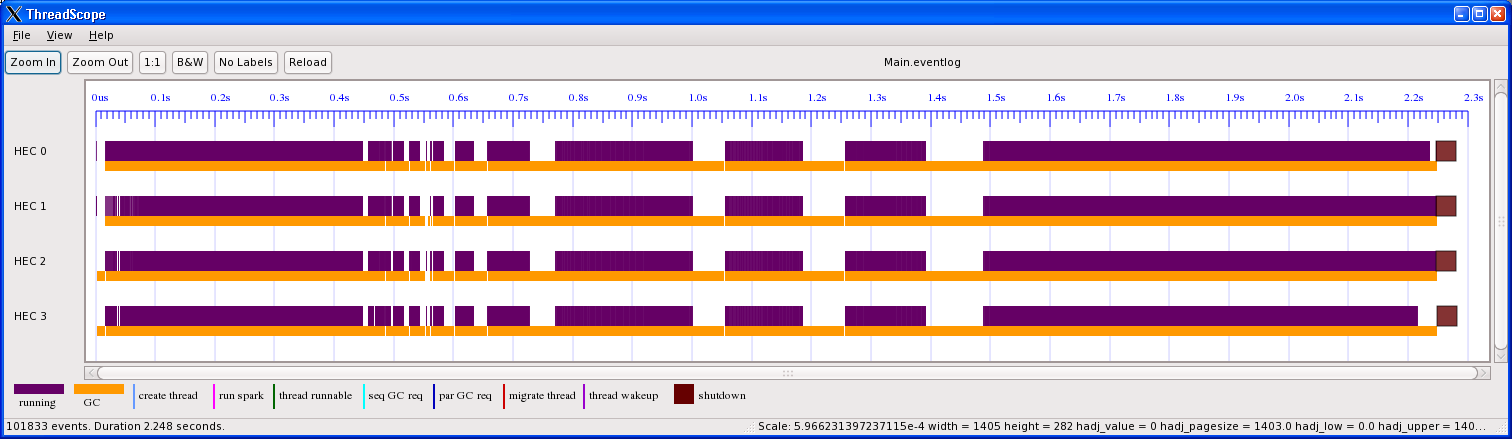
\includegraphics[scale=0.3]{soda1.png}
\end{center}
\caption{Soda ThreadScope profile}
\label{f:soda-threadscope}
\end{figure*}

\begin{figure*}
\begin{center}
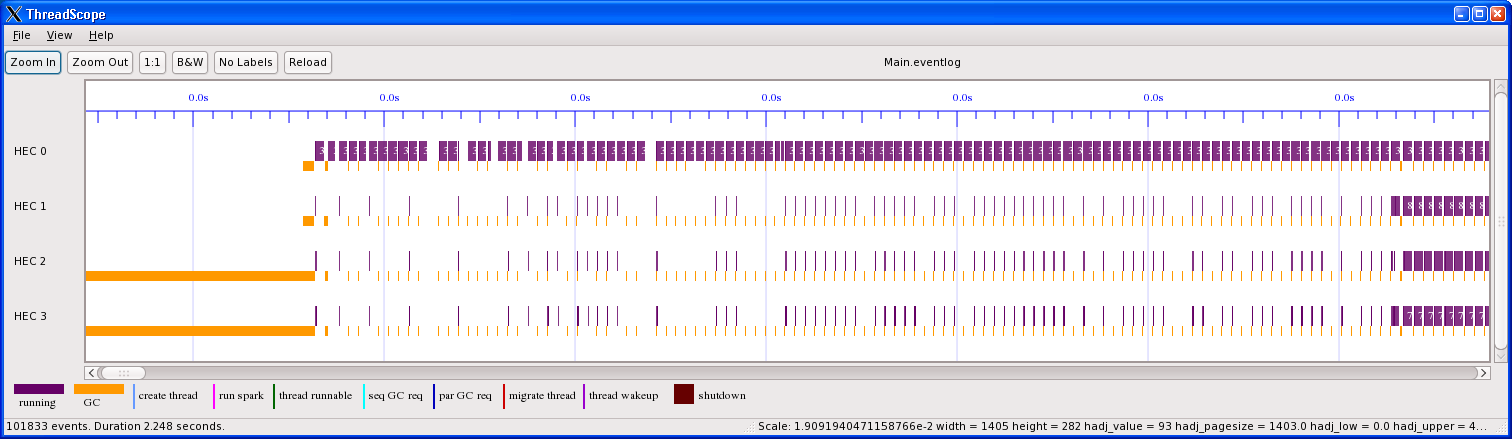
\includegraphics[scale=0.3]{soda2.png}
\end{center}
\caption{Soda ThreadScope profile (zoomed initial portion)}
\label{f:soda-threadscope2}
\end{figure*}

Figure~\ref{f:soda-threadscope} shows the ThreadScope profile for this
version of soda.  We can see that while an overall view of the runtime
shows a reasonable parallelisation, if we zoom into the initial part
of the run (Figure~\ref{f:soda-threadscope2}) we can see that HEC 0 is
running continuously, but threads on the other HECs are running very
briefly and then immediately getting blocked (zooming in further would
show the individual events).

Going back to the program, we can see that the grid of letters is
generated lazily by a function \codef{mk\_grid}.  What is happening here is
that the main thread creates sparks before the grid has been
evaluated, and then proceeds to evaluate the grid.  As each spark
runs, it blocks almost immediately waiting for the main thread to
complete evaluation of the grid.

This type of blocking is often not disastrous, since a thread will become
unblocked soon after the thunk on which it is blocking is evaluated
(see the discussion of ``blackholes'' in \citet{multicore-ghc}).  There
is nevertheless a short delay between the thread becoming runnable
again and the runtime noticing this and moving the tread to the run
queue.  Sometimes this delay can be hidden if the program has other
sparks it can be running in the meantime, but that is not the case
here.  There are also costs associated with blocking the thread and waking
it up again, which we would like to avoid if possible.

One way to avoid this is to evaluate the whole grid before creating
any sparks.  This is achieved by adding a call to \codef{rnf}:

\begin{lstlisting}
        -- force the grid to be evaluated:
        evaluate (rnf grid)
\end{lstlisting}

\begin{figure*}
\begin{center}
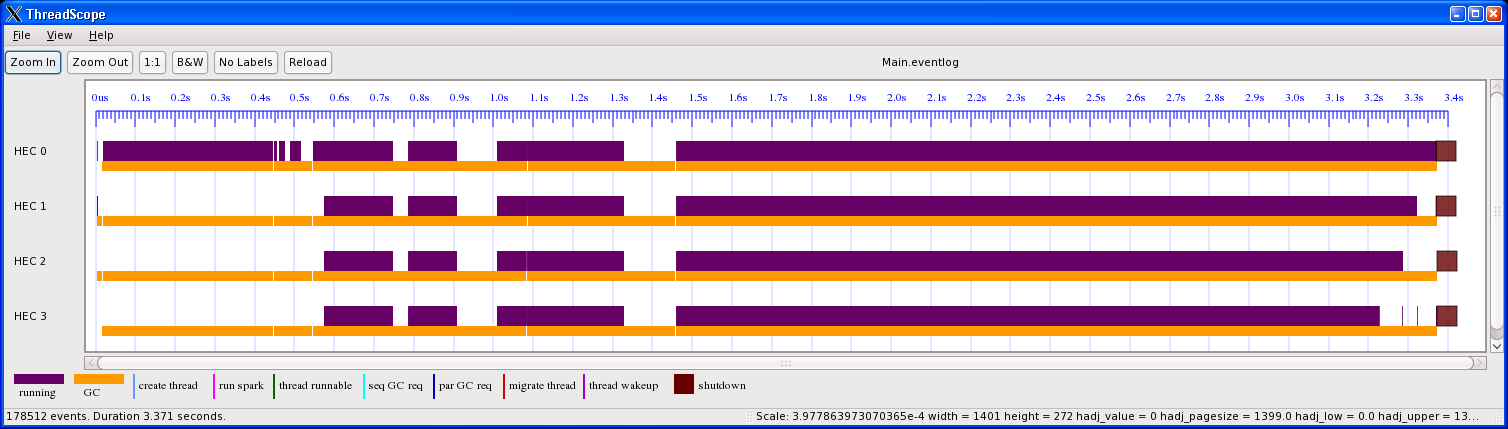
\includegraphics[scale=0.3]{soda3.png}
\end{center}
\caption{Soda ThreadScope profile (evaluating the input grid eagerly)}
\label{f:soda-threadscope3}
\end{figure*}

The effect on the profile is fairly dramatic
(Figure~\ref{f:soda-threadscope3}).  We can see that the parallel
execution doesn't begin until around 500ms into the execution:
creating the grid is taking quite a while.  The program also runs
slightly faster in parallel now:

\begin{verbatim}
  SPARKS: 12 (11 converted, 0 pruned)

  INIT  time    0.00s  (  0.00s elapsed)
  MUT   time    7.62s  (  2.31s elapsed)
  GC    time    3.35s  (  0.86s elapsed)
  EXIT  time    0.00s  (  0.00s elapsed)
  Total time   10.97s  (  3.18s elapsed)
\end{verbatim}
which we attribute to less blocking and unblocking of threads.  We can
also see that this program now has a significant sequential section -
around 15\% of the execution time - which limits the maximum speedup
we can achieve with 4 cores to 2.7, and we are already very close to
that at 2.5.

To improve parallelism further with this example we would have to
parallelise the creation of the initial grid; this probably isn't
hard, but it would be venturing beyond the realms of realism somewhat
to optimize the creation of the input data for a synthetic benchmark,
so we conclude the case study here.  It has been instructional to see
how thread blocking appears in the ThreadScope profile, and how to
avoid it by pre-evaluating data that is needed on multiple CPUs.

Here are a couple more factors that may be affecting the speedup we
see in this example:

\begin{itemize}
\item The static grid data is created on one CPU and has to be fetched
  into the caches of the other CPUs.  We hope in the future to be able
  to show the rate of cache misses (and similar characteristics) on
  each CPU alongside the other information in the ThreadScope profile,
  which would highlight issues such as this.
\item The granularity is too large: we can see that the HECs finish
  unevenly, losing a little parallelism at the end of the run.
\end{itemize}

\subsection{minimax}

Minimax is another historical Parallel Haskell program.  It is based
on an implementation of alpha-beta searching for the game tic-tac-toe,
from Hughes' influential paper ``Why Functional Programming Matters''
\cite{hughes:why-fp-matters}.  For the purposes of this paper we have generalised the
program to use a game board of arbitrary size: the original program
used a fixed 3x3 grid, which is too quickly solved to be a useful
parallelism benchmark nowadays.  However 4x4 still represents a
sufficient challenge without optimising the program further.

For the examples that follow, the benchmark is to evaluate the game
tree 6 moves ahead, on a 4x4 grid in which the first 4 moves have
already been randomly played.  This requires evaluating a maximum of
roughly 500,000,000 positions, although parts of the game tree will be
pruned, as we shall describe shortly.

We will explore a few different parallelisations of this program using
ThreadScope.  The function for calculating the best line in the game
is \codef{alternate}:

\begin{lstlisting}
alternate depth player f g board
 = move : alternate depth opponent g f board'
 where
   move@(board',_) = best f possibles scores
   scores          = map (bestMove depth opponent g f) possibles
   possibles       = newPositions player board
   opponent        = opposite player
\end{lstlisting}

This function calculates the sequence of moves in the game that give
the best outcome (as calculated by the alpha-beta search) for each
player.  At each stage, we generate the list of possible moves
(\codef{newPositions}), evaluate each move by alpha-beta search on the
game tree (\codef{bestMove}), and pick the best one (\codef{best}).

Let's run the program sequentially first to establish the baseline
runtime:

\begin{verbatim}
  14,484,898,888 bytes allocated in the heap

  INIT  time    0.00s  (  0.00s elapsed)
  MUT   time    8.44s  (  8.49s elapsed)
  GC    time    3.49s  (  3.51s elapsed)
  EXIT  time    0.00s  (  0.00s elapsed)
  Total time   11.94s  ( 12.00s elapsed)
\end{verbatim}

One obvious way to parallelise this problem is to evaluate each of the
possible moves in parallel.  This is easy to achieve with a
\codef{parListWHNF} strategy:

\begin{lstlisting}
  scores = map (bestMove depth opponent g f) possibles
             `using` parListWHNF
\end{lstlisting}

And indeed this does yield a reasonable speedup:

\begin{verbatim}
  14,485,148,912 bytes allocated in the heap

  SPARKS: 12 (11 converted, 0 pruned)

  INIT  time    0.00s  (  0.00s elapsed)
  MUT   time    9.19s  (  2.76s elapsed)
  GC    time    7.01s  (  1.75s elapsed)
  EXIT  time    0.00s  (  0.00s elapsed)
  Total time   16.20s  (  4.52s elapsed)
\end{verbatim}

\begin{figure*}
\begin{center}
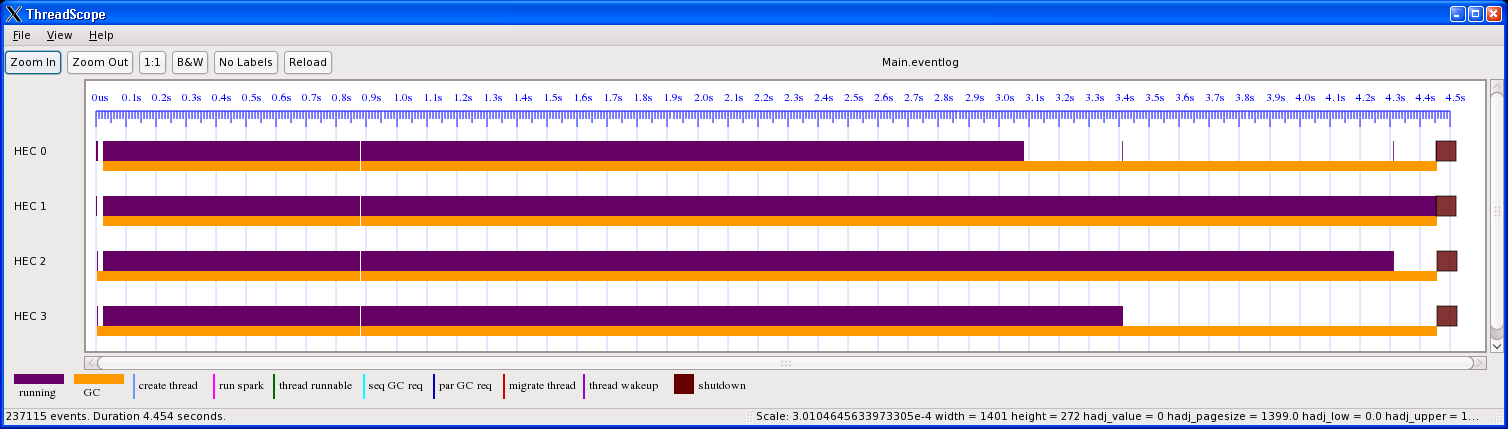
\includegraphics[scale=0.3]{minimax1.png}
\end{center}
\caption{Minimax ThreadScope profile}
\label{f:minimax-threadscope1}
\end{figure*}

A speedup of 2.7 on 4 processors is a good start!  However, looking at
the ThreadScope profile (Figure~\ref{f:minimax-threadscope1}), we can
see that there's a jagged edge on the right: our granularity is too
large, and we don't have enough work to keep all the processors busy
until the end.  What's more, as we can see from the runtime
statistics, there were only 12 sparks, corresponding to the 12
possible moves in the 4x4 grid after 4 moves have already been played.
In order to scale to more CPUs we will need to find more parallelism.

The game tree evaluation is defined as follows:

\begin{lstlisting}
bestMove :: Int -> Piece -> Player -> Player -> Board
         -> Evaluation
bestMove depth p f g 
  = mise f g 
  . cropTree
  . mapTree static
  . prune depth
  . searchTree p
\end{lstlisting}

Where \codef{searchTree} lazily generates a search tree starting
from the current position, with player \texttt{p} to play next.  The
function \codef{prune} prunes the search tree to the given depth, and
\codef{mapTree static} applies a static evaluation function to each
node in the tree.  The function \codef{cropTree} prunes branches below
a node in which the game has been won by either player.  Finally,
\codef{mise} performs the alpha-beta search, where \codef{f} and
\codef{g} are the min and max functions over evaluations for the
current player \codef{p}.

We must be careful with parallelisation here, because the algorithm is
relying heavily on lazy evaluation to avoid evaluating parts of the
game tree.  Certainly we don't want to evaluate beyond the prune
depth, and we also don't want to evaluate beyond a node in which one
player has already won (\codef{cropTree} prunes further moves after a win).
The alpha-beta search will prune even more of the tree: for example,
there is no point evaluating further down a branch if it has already
been established that there is a winning move.  So unless we are
careful, some of the parallelism we add here may be wasted
speculation.

The right place to parallelise is in the alpha-beta search itself.
Here is the sequential code:

\begin{lstlisting}
mise :: Player -> Player -> Tree Evaluation -> Evaluation
mise f g (Branch a []) = a
mise f g (Branch _ l) = foldr f (g OWin XWin) (map (mise g f) l)
\end{lstlisting}

The first equation looks for a leaf, and returns the evaluation of the
board at that point.  A leaf is either a completed game (either drawn
or a winning position for one player), or the result of pruning the
search tree.  The second equation is the interesting one: \codef{foldr
  f} picks the best option for the current player from the list of
evaluations at the next level.  The next level evaluations are given
by \codef{map (mise g f) l}, which picks the best options for the
\emph{other} player (which is why the \codef{f} and \codef{g} are
reversed).

The \codef{map} here is a good opportunity for parallelism.  Adding
a \codef{parListWHNF} strategy should be enough:

\begin{lstlisting}
mise f g (Branch _ l) = foldr f (g OWin XWin) 
                         (map (mise g f) l `using` parListWHNF)
\end{lstlisting}
However, this will try to parallelise every level of the search,
leading to some sparks with very fine granularity.  Also it may
introduce too much speculation: elements in each list after a win do
not need to be evaluated.  Indeed if we try this we get:

\begin{verbatim}
  22,697,543,448 bytes allocated in the heap

  SPARKS: 4483767 (639031 converted, 3457369 pruned)

  INIT  time    0.00s  (  0.01s elapsed)
  MUT   time   16.19s  (  4.13s elapsed)
  GC    time   27.21s  (  6.82s elapsed)
  EXIT  time    0.00s  (  0.00s elapsed)
  Total time   43.41s  ( 10.95s elapsed)
\end{verbatim}

We ran a lot of sparks (600k), but we didn't achieve much speedup over
the sequential version.
One clue that we are actually speculating useless work is the amount
of allocation.  In the sequential run the runtime reported 14GB
allocated, but this parallel version allocated 22GB\footnote{CPU time
  is not a good measure of speculative work, because in the parallel
  runtime threads can sometimes be spinning while waiting for work,
  particularly in the GC.}.

In order to eliminate some of the smaller sparks, we can
parallelise the alpha-beta to a fixed depth.  This is done by
introducing a new variant of \codef{mise}, \codef{parMise}, that
applies the \codef{parListWHNF} strategy up to a certain depth, and then
calls the sequential \codef{mise} beyond that.  Just using a depth of
one gives quite good results:

\begin{verbatim}
  SPARKS: 132 (120 converted, 12 pruned)

  INIT  time    0.00s  (  0.00s elapsed)
  MUT   time    8.82s  (  2.59s elapsed)
  GC    time    6.65s  (  1.70s elapsed)
  EXIT  time    0.00s  (  0.00s elapsed)
  Total time   15.46s  (  4.30s elapsed)
\end{verbatim}

\begin{figure*}
\begin{center}
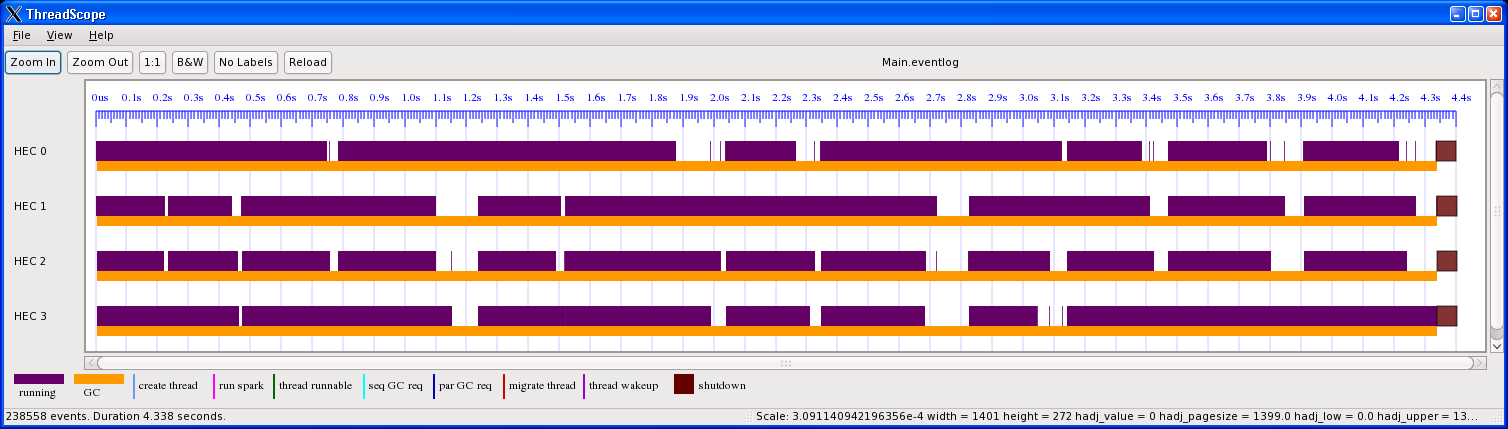
\includegraphics[scale=0.3]{minimax2.png}
\end{center}
\caption{Minimax ThreadScope profile (with parMise 1)}
\label{f:minimax-threadscope2}
\end{figure*}

Though as we can see from the ThreadScope profile
(Figure~\ref{f:minimax-threadscope2}), there are some gaps.
Increasing the threshold to two works nicely:

\begin{verbatim}
  SPARKS: 1452 (405 converted, 1046 pruned)

  INIT  time    0.00s  (  0.03s elapsed)
  MUT   time    8.86s  (  2.31s elapsed)
  GC    time    6.32s  (  1.57s elapsed)
  EXIT  time    0.00s  (  0.00s elapsed)
  Total time   15.19s  (  3.91s elapsed)
\end{verbatim}

\begin{figure*}
\begin{center}
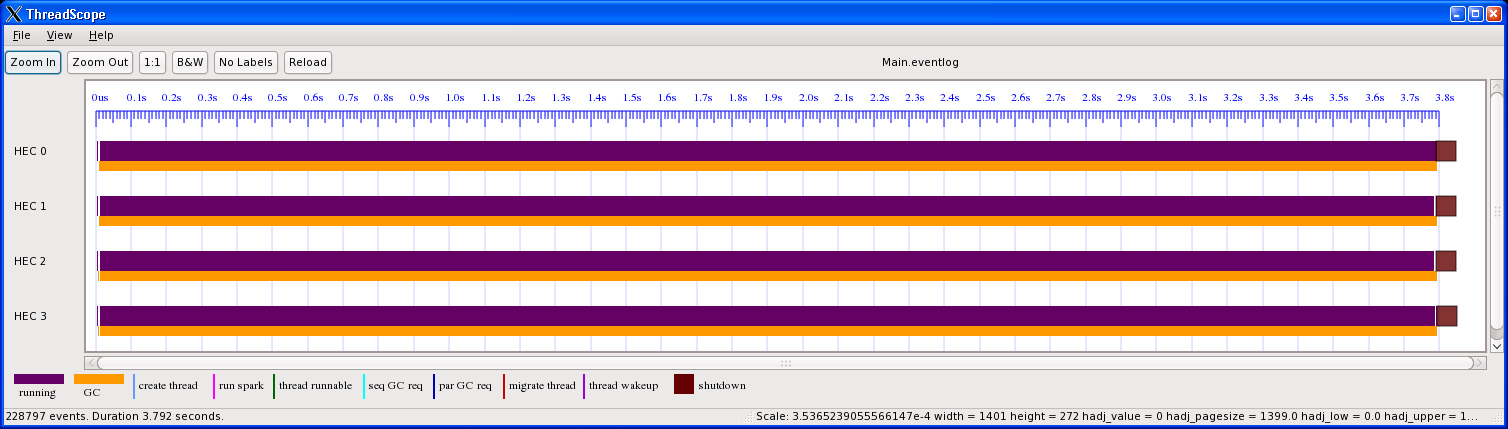
\includegraphics[scale=0.3]{minimax3.png}
\end{center}
\caption{Minimax ThreadScope profile (with parMise 2)}
\label{f:minimax-threadscope3}
\end{figure*}

We have now achieved a speedup of 3.1 on 4 cores against the
sequential code, and as we can see from the final ThreadScope profile
(Figure~\ref{f:minimax-threadscope3}) all our cores are kept busy.

We found that increasing the threshold to 3 starts to cause
speculation of unnecessary work.  In 4x4 tic-tac-toe most positions
are a draw, so it turns out that there is little speculation in the
upper levels of the alpha-beta search, but as we get deeper in the
tree, we find positions that are a certain win for one player or
another, which leads to speculative work if we evaluate all the moves
in parallel.  

Ideally GHC would have better support for speculation: right now,
speculative sparks are not garbage collected when they are found to be
unreachable.  We do plan to improve this in the future, but
unfortunately changing the GC policy for sparks is incompatible with
the current formulation of Strategies \cite{multicore-ghc}.

\subsection{Thread Ring}

The thread ring benchmark originates in the Compter Language
Benchmarks Game\footnote{\url{http://shootout.alioth.debian.org/}}
(formerly known as the Great Computer Language Shootout).  It is a
simple concurrency benchmark, in which a large number of threads are
created in a ring topology, and then messages are passed around the
ring.  The code for our version of the benchmark is given in
Figure~\ref{f:threadring-code}.  In fact this version uses a linear
string of threads rather than a ring.  A number of messages are pumped
in to the first thread in the string, and then collected at the other
end.

\begin{figure}
\begin{lstlisting}
import Control.Concurrent
import Control.Monad
import System
import GHC.Conc (forkOnIO)

thread :: MVar Int -> MVar Int -> IO ()
thread inp out = do 
  x <- takeMVar inp
  putMVar out $! x+1
  thread inp out

spawn cur n = do 
  next <- newEmptyMVar
  forkIO $ thread cur next
  return next

main = do 
  n <- getArgs >>= readIO.head
  s <- newEmptyMVar
  e <- foldM spawn s [1..2000]
  f <- newEmptyMVar
  forkIO $ replicateM n (takeMVar e) >>= putMVar f . sum
  replicateM n (putMVar s 0)
  takeMVar f
\end{lstlisting}
\caption{ThreadRing code}
\label{f:threadring-code}
\end{figure}

Our aim is to try to make this program speed up in parallel.  We
expect there to be parallelism available: multiple messages are
being pumped through the thread string, so we ought to be able to pump
messages through distinct parts of the string in parallel.

First, the sequential performance.  This is for 500 messages and 2000 threads:

\begin{verbatim}
  INIT  time    0.00s  (  0.00s elapsed)
  MUT   time    0.18s  (  0.19s elapsed)
  GC    time    0.01s  (  0.01s elapsed)
  EXIT  time    0.00s  (  0.00s elapsed)
  Total time    0.19s  (  0.21s elapsed)
\end{verbatim}

Next, running the program on two cores:

\begin{verbatim}
  INIT  time    0.00s  (  0.00s elapsed)
  MUT   time    0.65s  (  0.36s elapsed)
  GC    time    0.02s  (  0.01s elapsed)
  EXIT  time    0.00s  (  0.00s elapsed)
  Total time    0.67s  (  0.38s elapsed)
\end{verbatim}

\begin{figure*}
\begin{center}
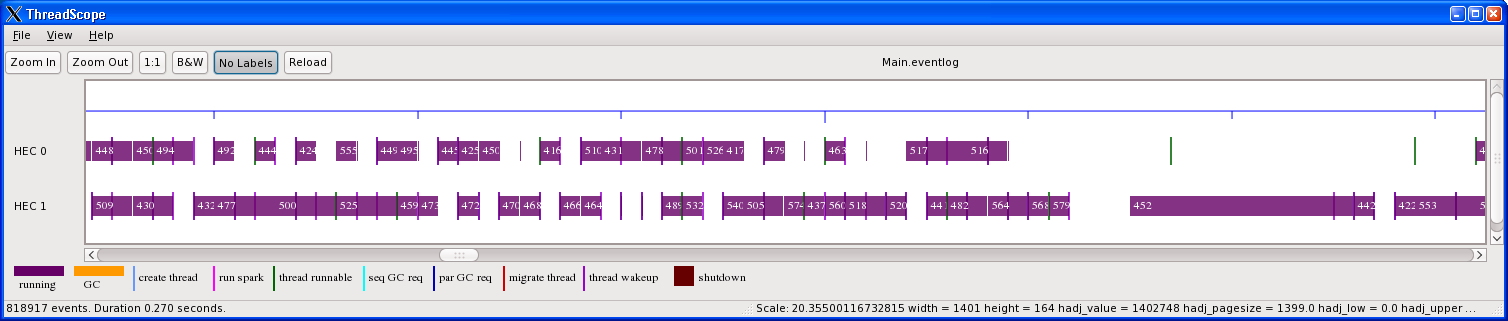
\includegraphics[scale=0.3]{threadring1.png}
\end{center}
\caption{ThreadRing profile (no explicit placement; zoomed in)}
\label{f:threadring1}
\end{figure*}

Things are significantly slower when we add a core.  Let's examine the
ThreadScope profile to see why - at first glance, the program seems to
be using both cores, but as we zoom in we can see that there are lots
of gaps (Figure~\ref{f:threadring1}).  

In this program we want to avoid communication between the two
separate cores, because that will be expensive.  We want as much
communication as possible to happen between threads on the same core,
where it is cheap.  In order to do this, we have to give the scheduler
some help: we know the structure of the communication in this program,
so we can place threads optimally to take advantage of that.  GHC
provides a way to place a thread onto a particular core (or HEC),
using the \codef{forkOnIO} operation.  The placement scheme we use is
to divide the string into linear segments, one segment per core (in
our case two).

This strategy gets us back to the same performance as the sequential
version:

\begin{verbatim}
  INIT  time    0.00s  (  0.00s elapsed)
  MUT   time    0.23s  (  0.19s elapsed)
  GC    time    0.02s  (  0.02s elapsed)
  EXIT  time    0.00s  (  0.00s elapsed)
  Total time    0.26s  (  0.21s elapsed)
\end{verbatim}

\begin{figure*}
\begin{center}
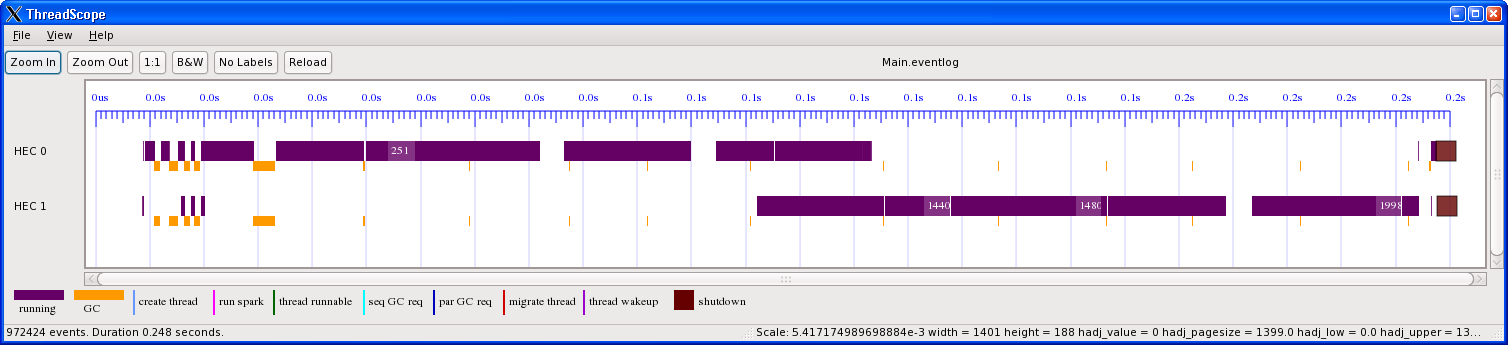
\includegraphics[scale=0.3]{threadring2.png}
\end{center}
\caption{ThreadRing profile (with explicit placement)}
\label{f:threadring2}
\end{figure*}

Why don't we actually see any speedup?
Figure~\ref{f:threadring2} shows the ThreadScope profile.
The program has now been almost linearized; there is a small amount of
overlap, but most of the execution is sequential, first on one core
and then the other.

\begin{figure*}
\begin{center}
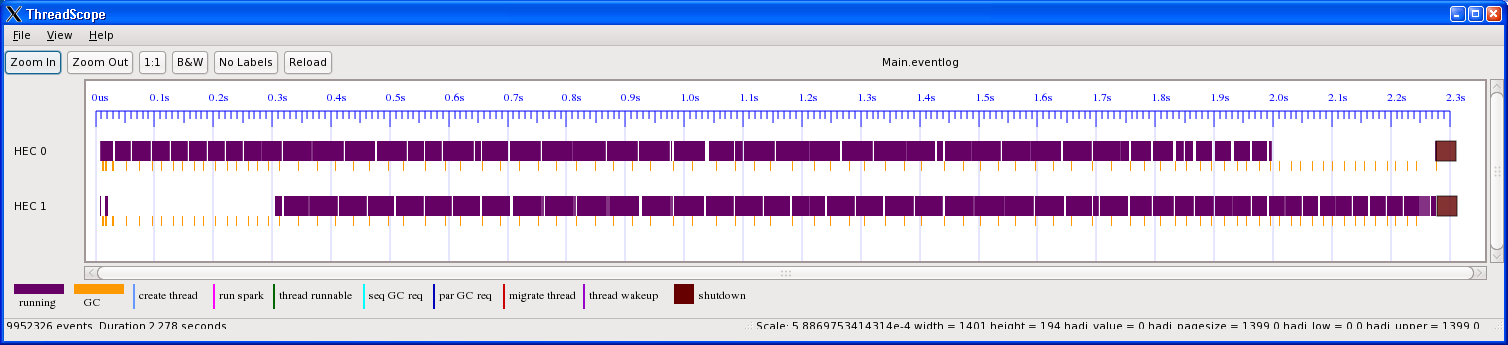
\includegraphics[scale=0.3]{threadring3.png}
\end{center}
\caption{ThreadRing profile (explicit placement and more messages)}
\label{f:threadring3}
\end{figure*}

Investigating the profile in more detail shows that this is a
scheduling phenomenon.  The runtime has moved all the messages through
the first string before it propagates any into the second string, and
this can happen because the total number of messages we are using for
the benchmark is less than the number of threads.  If we increase the
number of messages, then we do actually see more parallelism;
Figure~\ref{f:threadring3} shows the execution profile for 2000
messages and 2000 threads.


% $Id: related-work.tex#1 2009/04/22 10:31:00 REDMOND\\satnams $
% $Source: //depot/satnams/haskell/ThreadScope/papers/haskell_symposium_2009/related-work.tex $

\section{Related Work}
GranSim~\cite{loidl} is an event-driven simulator for the parallel execution of Glasgow Parallel Haskell (GPH) programs which allows the parallel behaviour of Haskell programs to be analyzed by instantiating any number of virtual processors which are emulated by a single thread on the host machine. GranSim has an associated set of visualization tools which show overall activity, per-processor activity, and per-thread activity. There is also a sepatate tool for analyzing the granularity of the generated threads.

\section{Conclusions and Further work}
\label{s:conclusion}
We have shown how thread-based profile information can be effectively
used to help understand and fix parallel performance bugs in 
semi-explicitly parallel Haskell programs. Many of the techniques
we present in this paper are also applicable to other kinds of
concurrent and parallel Haskell programs e.g. programs that
explicitly create threads through \codef{forkIO} and synchronize
through \codef{MVars} as well as programs that use atomic blocks
implemented by software transactional memory. Furthermore, we expect
the profiling techniques in this paper to be of great benefit to
developers using Data Parallel Haskell. 

The ability to profile parallel Haskell programs plays an important
part in the development of such programs because the analysis
process motivates the need to develop specialized strategies to
help control evaluation order, extent and granularity as we demonstrated in
the minmax example.

Here are some of the future directions we would like to take this
work:

\begin{itemize}
\item Improve the user interface and navigation of ThreadScope.  For
  example, it would be nice to filter the display to show just a
  subset of the threads, in order to focus on the behaviour of a
  particular thread or group of threads.

\item It would also be useful to understand how threads interact with each 
   other via \codef{MVars} e.g. to make it easier to see which 
   threads are blocked on read and write accesses to \codef{MVar}s.

\item The programmer should be able to generate events
  programmatically, in order to mark positions in the timeline so that
  different parts of the program's execution can easily be identified
  and separated in ThreadScope.

\item It would be straightforward to produce graphs similar to those
  from the GpH programming tools \cite{gph}.

\item Combine the timeline profile with information from the OS and
  CPU.  For example, for IO-bound concurrent programs we might like to
  see IO or network activity displayed on the timeline.  Information
  from CPU performance counters could also be superimposed or
  displayed alongside the thread timelines, providing insight into
  cache behaviour, for example.

\item Have the runtime system generate more tracing information, so
  that ThreadScope can display information about such things as memory
  usage, run queue sizes, spark pool sizes, and foreign call activity.
\end{itemize}

The authors would like to acknowledge the work of the developers
of previous Haskell concurrent and parallel profiling systems
which have provided much inspiration for our own work. Specifically
work on GpH, GranSim and Eden was particularly useful.

{\small
\bibliographystyle{plainnat}
\bibliography{ghc-parallel-tuning}
}

\end{document}
